\documentclass[ignorenonframetext,xcolor=pdftex,dvipsnames,table]{beamer}
\mode<article>{\usepackage[svgnames]{xcolor}
\usepackage[colorlinks=true]{hyperref}
\setlength{\textwidth}{180mm}
\setlength{\oddsidemargin}{-1cm}
\setlength{\evensidemargin}{-1cm}
%\setlength{\topmargin}{-40pt}
}
\mode<presentation>{
\usetheme{Madrid}
\setbeamercovered{transparent}
% or whatever (possibly just delete it)
%\AtBeginSubsection[]
%{
%  \begin{frame}<beamer>{Outline}
%    \tableofcontents[currentsection,currentsubsection]
%  \end{frame}
%}
%%%Configure section names to appear in beamer
\setbeamertemplate{headline}
{%
\begin{beamercolorbox}{section in head/foot}
\vskip2pt\insertsection$\to$\insertsubsection\vskip2pt
\end{beamercolorbox}%
}
%\usepackage[svgnames]{xcolor}
%%paginacion
\usefoottemplate{\hfill \insertframenumber{}}% /\inserttotalframenumber}
%delete the navigation buttons
\setbeamertemplate{navigation symbols}{}
}
% everyone:

\usepackage[utf8]{inputenc}
%\usepackage{textcomp}
\usepackage[spanish]{babel}
\spanishdecimal{.}
\addto\captionsspanish{%
\def\tablename{Tabla}%
}
\usepackage{amsmath}
\usepackage{amssymb}
\usepackage{amsthm}
%%%%%%%%%%from beyond.tex
\usepackage{cancel}
\usepackage{simplewick}
\usepackage[toc,page]{appendix}
\usepackage{comment}
\includecomment{inprogress}
\specialcomment{inprogress}
{\begingroup\itshape \textbf{Begin Draft:}}{\textbf{End Draft.} \medskip \endgroup}
%\excludecomment{inprogress}

\def\lt{<} % compatibility with instiki
\def\gt{>} % compatibility with instiki
%%%%%%%%%%%%%%%%%%%%%%
%\usepackage[colorlinks=true]{hyperref}
\usepackage{graphicx}
%\usepackage{color}
\usepackage{bm}
\usepackage{framed}
\definecolor{shadecolor}{named}{gray}
\newcommand{\filetitle}[1]{
\begin{shaded}
\noindent{\color{white}#1}
\end{shaded}}


\graphicspath{{figures/}}
%%%%%%%%%%%%%%%%%%%%listings%%%%%%%%%%%%%%%
\usepackage{listings}
%\usepackage{listingsutf8}

\usepackage{caption}
\DeclareCaptionFont{white}{\color{white}}
\DeclareCaptionFormat{listingm}{\colorbox{gray}{\parbox{\textwidth}{#1#2#3}}}
\DeclareCaptionFormat{listingmm}{\colorbox{gray}{\parbox{\textwidth}{Hola #3}}}
\DeclareCaptionFormat{ipython}{\colorbox{lightgray}{\parbox{\textwidth}{\centering IPython}}}
\DeclareCaptionFormat{terminal}{\parbox[t]{\textwidth}{\centering \fbox{Terminal}}}
\captionsetup[lstlisting]{format=listingm,labelfont=white,textfont=white}
%%%%%%%%%%%%%%%%%%%%%%%%%%%%%%%%%%%%%%%%%%
%\usepackage{bbold}
\newenvironment{pyprogram}{\captionsetup[lstlisting]{format=listingm,labelfont=white,textfont=white}
\lstset{frame=bl}}
{}
\newenvironment{pysnippet}{\captionsetup[lstlisting]{format=listingm,labelfont=white,textfont=white}}{}
\newenvironment{ipython}{\captionsetup[lstlisting]{format=ipython}
\lstset{columns=fixed}}{}
\newenvironment{pysample}{\captionsetup[lstlisting]{format=ipython}
\lstset{frame=tb}
}{}
\newenvironment{terminal}{\captionsetup[lstlisting]{format=terminal}
\lstset{language=bash,backgroundcolor=\color{lightgray},belowcaptionskip=-0pt,columns=fixed}
}{}
%\newenvironment{ejemplo}{}{}

 \lstset{language=python
%,inputencoding=utf8
%,showspaces=false
%{\small Hola} {\footnotesize Hola} {\scriptsize Hola} {\tiny Hola}
,basicstyle=\small\ttfamily
%,basicstyle=\small\sffamily,
,keywordstyle=\color{blue}
,commentstyle=\normalfont\ttfamily\color{red}
,stringstyle=\color{Green}
%,numbers=left
%,numberstyle=\tiny
,frame=b
,inputencoding=utf8
,extendedchars=true
,columns=fullflexible
,showstringspaces=false
%,backgroundcolor=\color{lightgray}
,texcl=true
}

\newcommand{\timesm}{\times}
\newtheorem{ejemplo}[theorem]{Ejemplo}

\newcommand{\chapter}{}
\newcommand{\ignore}[1]{}
\begin{document}
%%Comment the following two lines for full processing
%\mode<presentation>{\input{cf_tmp}}
%\end{document}

\mode<presentation>{
\chapter{Introducci\'on}
\label{chap:1}


%%% Local Variables: 
%%% mode: latex
%%% TeX-master: "mecanica"
%%% End: 
}
\mode<presentation>{
\chapter{Movimiento circular}
\label{chap:cin1}



% \subsection{Caida libre}
% La observaci\'on experimental, como por ejemplo la caida de una pluma y un bal\'\i n en un tubo de vacio, han establecido que todos los objetos cerca a la tierra se aceleran al la misma tasa constante cuando otros efectos externos est\'an excluidos.


% En un sistema de coordenadas donde la direcci\'on de movimiento es perpendicular a la superficie de la tierra, podemos definir un \emph{vector unitario}, es decir, un vector de magnitud 1 y direcci\'on positiva como $\hat{\mathbf{j}}$, tal que
% \begin{align}
%   |\hat{\mathbf{j}}| = 1,
% \end{align}
% donde los simbolos $|\ |$ representan la magnitud del vector. Entonces el vector de aceleraci\'on gravitacional se puese escribir como
% \begin{align}
%   \mathbf{a}=-g \hat{\mathbf{j}}\,.
% \end{align}

% Los vectores se denotan con letra negrilla o con una flecha arriba $\vec a$. Usaremos la primera opci\'on en este texto. La magnitud del vector de aceleraci\'on gravitacional es entonces:
% \begin{align}
%   |\mathbf{a}|=g=9.8\ \frac{\text{m}}{\text{s}}
% \end{align}

% La soluci\'on a la ecuaci\'on de movimiento
% \begin{align}
%   \frac{d^2y(t)}{dt^2}=-g\,,
% \end{align}

% % ver notas Kowalaski 3-11


\section{Movimiento Circular Uniforme}

Considere el movimiento descrito por la siguiente ecuaci\'on
\begin{align}
  \label{eq:mua}
  \mathbf{r}(t)=r\left(\hat{\mathbf{i}}\cos(\omega t)+\hat{\mathbf{j}}\sin(\omega t)\right),
\end{align}
con $r=\text{constante}$ y $\omega=\text{constante}$, representado en la figura~\ref{fig:mua1}.

La velocidad es
\begin{align}
  \mathbf{v}=&%detalles\\
  r\omega\left(-\hat{\mathbf{i}}\sin(\omega t)+\hat{\mathbf{j}}\cos(\omega t)\right),
\end{align}
representado en la figura~\ref{fig:mua2}. Note que $\mathbf{r}\cdot\mathbf{v}=0$, de modo que los vectores son perpendiculares.

La aceleraci\'on es
\begin{align}
  \mathbf{a}=&%detalles\\
  -r\omega^2\left(\hat{\mathbf{i}}\cos(\omega t)+\hat{\mathbf{j}}\sin(\omega t)\right),
\end{align}
representado en la figura~\ref{fig:mua3}. Note que $\mathbf{a}\cdot\mathbf{v}=0$, de modo que los vectores son perpendiculares. Adem\'as
$\mathbf{r}\cdot\mathbf{a}=-1$, de modo que los vectores son antiparalelos.


\begin{frame}[fragile,allowframebreaks]
  \begin{figure}
    \centering
    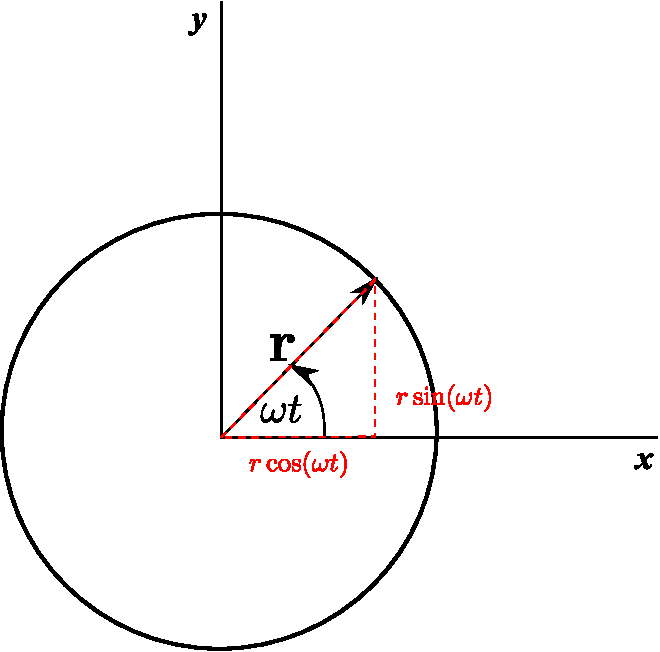
\includegraphics[scale=0.65]{mua1}    
    \caption{Posici\'on}
    \label{fig:mua1}
  \end{figure}

\end{frame}
\begin{frame}[fragile,allowframebreaks]
  \begin{figure}
    \centering
    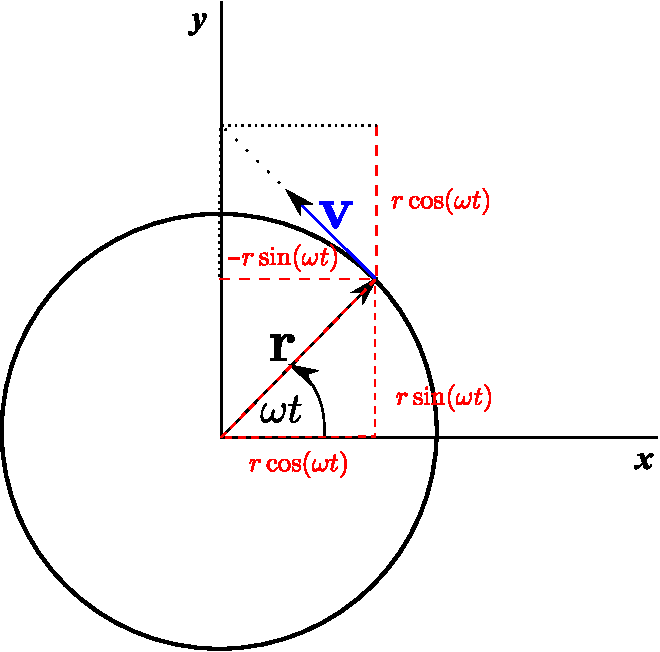
\includegraphics[scale=0.65]{mua2}    
    \caption{Velocidad: tangente a la curva}
    \label{fig:mua2}
  \end{figure}
\end{frame}

\begin{frame}[fragile,allowframebreaks]
  \begin{figure}
    \centering
    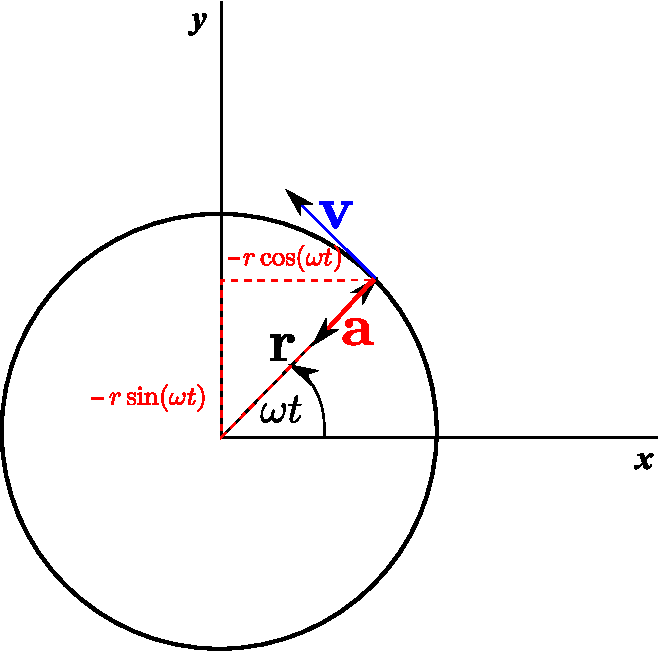
\includegraphics[scale=0.65]{mua3}
    \caption{Aceleraci\'on: centr\'\i peta}
    \label{fig:mua3}
  \end{figure}


\end{frame}

\subsection{Movimiento generalizado en coordenadas polares}
La ecuaci\'on para el vector de posici\'on puede escribirse en general como
\begin{align}
\label{eq:rpol}
  \mathbf{r}(t)=r(t)\left(\hat{\mathbf{i}}\cos[\theta(t)]+\hat{\mathbf{j}}\sin[\theta(t)]\right)\,.
\end{align}
Para algunos problemas es conveniente reescribir \'esta ecauaci\'on en coordenadas polares:
\begin{inprogress}
  Faltan detalles
\end{inprogress}
\begin{align}
  \label{eq:polinv}
  \begin{pmatrix}
    \hat{\mathbf{r}}\\
    \hat{\boldsymbol{\theta}}
  \end{pmatrix}=
  \begin{pmatrix}
    \cos\theta&-\sin\theta\\
    \sin\theta&\cos\theta\\
  \end{pmatrix}
  \begin{pmatrix}
    \;\hat{\mathbf{i}}\;\\
    \hat{\mathbf{j}}\\
  \end{pmatrix}.
\end{align}
con inverso
\begin{align}
  \begin{pmatrix}
    \;\hat{\mathbf{i}}\;\\
    \hat{\mathbf{j}}\\
  \end{pmatrix}=
  \begin{pmatrix}
    \cos\theta&-\sin\theta\\
    \sin\theta&\cos\theta\\
  \end{pmatrix}
  \begin{pmatrix}
    \hat{\mathbf{r}}\\
    \hat{\boldsymbol{\theta}}
  \end{pmatrix}.
\end{align}

La velocidad es
\begin{align}
  \label{eq:vpol}
  \mathbf{v}(t)=&%detalles\\
  \dot{r}(t)\hat{\mathbf{r}}(t)+r(t)\dot{\theta}(t)\hat{\boldsymbol{\theta}}(t)\,.
\end{align}
y la aceleraci\'on es
\begin{align}
\label{eq:apol}
  \mathbf{a}(t)=&%detalles\\
[\underbrace{\ddot{r}(t)}_{{\text{Acel. lineal.}}}
-\underbrace{r(t)\dot{\theta}^2(t)}_{{\text{Acel. centr\'\i peta.}}}]\hat{\mathbf{r}}(t)
+[\underbrace{r(t)\ddot{\theta}(t)}_{{\text{Acel. lineal tangencial.}}}
+\underbrace{2\dot{r}(t)\dot{\theta}(t)}_{{\text{Acel. de coriolis.}}}]\hat{\boldsymbol{\theta}}(t).
\end{align}
\begin{itemize}
\item[\textbf{Ejemplo}] \textbf{MCU}:\\
Comparando (\ref{eq:mua}) con (\ref{eq:rpol}), tenemos para el Movimiento Circular Uniforme que
\begin{align}
  \label{eq:muapol}
   \dot{r}=&0&&&&\\
  \theta(t)=&\omega t\,,&\dot{\theta}(t)=&\omega\,,&\ddot{\theta}(t)=&0\,.
\end{align}
De modo que reemplazando las ecuaciones \eqref{eq:muapol} en las ecuaciones \eqref{eq:vpol}, \eqref{eq:apol}, y usando la transformaci\'on inversa \eqref{eq:polinv}, tenemos que
\begin{align}
  \mathbf{r}(t)=&r\hat{\mathbf{r}}(t)\nonumber\\
  =&r\left(\hat{\mathbf{i}}\cos(\omega t)+\hat{\mathbf{j}}\sin(\omega t)\right),
\end{align}
\begin{align}
    \mathbf{v}(t)=&r\omega\hat{\boldsymbol{\theta}}(t)\nonumber\\
    =&r\omega\left(-\hat{\mathbf{i}}\sin(\omega t)+\hat{\mathbf{j}}\cos(\omega t)\right),
\end{align}
\begin{align}
  \mathbf{a}(t)=&-r\omega^2\hat{\mathbf{r}}(t)\nonumber\\
  =&-r\omega^2\left(\hat{\mathbf{i}}\cos(\omega t)+\hat{\mathbf{j}}\sin(\omega t)\right),
\end{align}
de modo que en el MCU la velocidad no tiene componente radial, y s\'olo
contribuye la aceleraci\'on centr\'\i peta, como era de esperarse.
\end{itemize}

Continuara...

%\left(\right)
%ver inkscape vectores primera capa






%%% Local Variables: 
%%% mode: latex
%%% TeX-master: "mecanica"
%%% End: 

}
%\mode<presentation>{\input{bibliography}}

\end{document}

%TEMPLATES:

\chapter{Hola}
\section{Introduction}
This is the introduction text. This text is not shown in the
presentation, but will be part of the article.
\begin{frame}
Hola mundo
\end{frame}
This text is once more not shown in the presentation.
\section{Main Part}
While this text is not shown in the presentation, the section command
also applies to the presentation.
We can add a subsection that is only part of the article like this:
\subsection<article>{Article-Only Section}
With some more text.
\begin{frame}
This text is part both of the article and of the presentation.
\begin{itemize}
\item This stuff is also shown in both version.
\item This too.
\only<article>{\item This particular item is only part
of the article version.}
\item<presentation:only@0> This text is also only part of the article.
\end{itemize}

\end{frame}

Templates:
%%%tablas de colores
\mode<presentation>{\rowcolors{1}{RoyalBlue!20}{}}

\begin{frame}[fragile,allowframebreaks]
\end{frame}

%numbers in beamer
\begin{lstlisting}[numbers=left,xleftmargin=1cm,numberstyle=\tiny,escapeinside={(*}{*)}]
\end{lstlisting}


\begin{pyprogram}
\lstset{numbers=left}
\begin{lstlisting}[label=XXX,caption=XXX]
\end{lstlisting}
\end{pyprogram}

\begin{pyprogram}
\mode<presentation>{\lstset{basicstyle=\tiny\ttfamily}}
\filetitle{cinematica.py}
\lstinputlisting{python/programas/cinematica/cinematica.py}
\end{pyprogram}



\begin{ipython}
\begin{lstlisting}[title=]
In [1]:
\end{lstlisting}
\end{ipython}

\begin{terminal}
\begin{lstlisting}[title=1]

\end{lstlisting}
\end{terminal}

\begin{columns}
  \begin{column}{0.5\textwidth}
    
  \end{column}
  \begin{column}{0.5\textwidth}
    
  \end{column}
\end{columns}


%%% Local Variables: 
%%% mode: latex
%%% TeX-master: "mecanica.beamer.tex"
%%% End: 
